%header and footer for separate chapter files

\ifx\whole\undefined
\documentclass[12pt, leqno]{book}
\usepackage{graphicx}
\usepackage{eps-to-pdf}
\input style-for-curves.sty
%\input sl-macros.sty
\usepackage{hyperref}
\usepackage{showkeys} %This shows the labels.
\usepackage{msribib}
\usepackage{pdfpages}
\usepackage{draftwatermark}
\SetWatermarkText{DRAFT:\ \today}
\SetWatermarkScale{2}
\SetWatermarkColor[gray]{0.9}

%\usepackage{SLAG,msribib,local}
%\usepackage{amsmath,amscd,amsthm,amssymb,amsxtra,latexsym,epsfig,epic,graphics}
%\usepackage[matrix,arrow,curve]{xy}
%\usepackage{graphicx}
%\usepackage{diagrams}
%
%%\usepackage{amsrefs}
%%%%%%%%%%%%%%%%%%%%%%%%%%%%%%%%%%%%%%%%%%
%%\textwidth16cm
%%\textheight20cm
%%\topmargin-2cm
%\oddsidemargin.8cm
%\evensidemargin1cm
%
%%%%%%Definitions
%\input preamble.tex
%\input style-for-curves.sty
%\def\TU{{\bf U}}
%\def\AA{{\mathbb A}}
%\def\BB{{\mathbb B}}
%\def\CC{{\mathbb C}}
%\def\QQ{{\mathbb Q}}
%\def\RR{{\mathbb R}}
%\def\facet{{\bf facet}}
%\def\image{{\rm image}}
%\def\cE{{\cal E}}
%\def\cF{{\cal F}}
%\def\cG{{\cal G}}
%\def\cH{{\cal H}}
%\def\cHom{{{\cal H}om}}
%\def\h{{\rm h}}
% \def\bs{{Boij-S\"oderberg{} }}
%
%\makeatletter
%\def\Ddots{\mathinner{\mkern1mu\raise\p@
%\vbox{\kern7\p@\hbox{.}}\mkern2mu
%\raise4\p@\hbox{.}\mkern2mu\raise7\p@\hbox{.}\mkern1mu}}
%\makeatother

%%
%\pagestyle{myheadings}

%\input style-for-curves.tex
%\documentclass{cambridge7A}
%\usepackage{hatcher_revised} 
%\usepackage{3264}
   
\errorcontextlines=1000
%\usepackage{makeidx}
\let\see\relax
\usepackage{makeidx}
\makeindex
% \index{word} in the doc; \index{variety!algebraic} gives variety, algebraic
% PUT a % after each \index{***}

\overfullrule=5pt
\catcode`\@\active
\def@{\mskip1.5mu} %produce a small space in math with an @

\title{A Chapter from ``The Practice of Algebraic Curves"}
\author{\copyright David Eisenbud and Joe Harris}
%%\includeonly{%
%0-intro,01-ChowRingDogma,02-FirstExamples,03-Grassmannians,04-GeneralGrassmannians
%,05-VectorBundlesAndChernClasses,06-LinesOnHypersurfaces,07-SingularElementsOfLinearSeries,
%08-ParameterSpaces,
%bib
%}

\date{\today}
%%\date{}
%\title{Curves}
%%{\normalsize ***Preliminary Version***}} 
%\author{David Eisenbud and Joe Harris }
%
%\begin{document}

\begin{document}
\maketitle

\pagenumbering{roman}
\setcounter{page}{5}
%\begin{5}
%\end{5}
\pagenumbering{arabic}
\tableofcontents
\fi


\chapter{Inflection points}\label{inflections chapter}
\label{InflectionsChapter}

Generalizing the ramification points of a map from a smooth curve $C$
\index{flex|see inflection point}%
to $\PP^1` `$, there are finitely many ``special'' points determined by
any linear series on any curve, the \emph{inflection points}.
\index{inflection point}%
We love this topic for its echoes of classical algebraic geometry and
it will provide the tools to give a proof of the Brill--Noether
theorem in the following chapter. In characteristic 0 every linear
series has finitely many inflection points, and the number of these,
properly counted, depends only on the genus of the curve and the
degree of the linear series.

\section{Inflection points,  Pl\"ucker formulas and Weierstrass points}

\subsection*{Definitions}
To characterize the inflection points of a linear series 
$\sD = (\sL, V)$ on a curve $C$, we will use the following result:

\begin{proposition}\label{vanishing sequence} Let $V$ be a
\index{vanishing sequence}%
  finite-dimensional vector space of 
global sections
\index{global section}%
of an 
invertible sheaf
\index{invertible sheaf}%
$\sL$ on a smooth curve $C$, and let $p \in C$
be a point. There exists a basis $\sigma_0, \dots, \sigma_r$ of $V$
consisting of sections vanishing to different orders at~$p$. Thus the set 
$$
\{ \ord_p(\sigma) \mid \sigma \neq 0 \in V \}
$$
 has cardinality $\dim V` `$.
\unif
\end{proposition}

\begin{proof} 
Let $\tau_0, \dots, \tau_r$ be any basis of $V` `$.  If  $\tau_i$ and
$\tau_j$ vanish to the same order at~$p$, then
some nonzero linear combination $\tau_i' \colonequals  a\tau_i+b\tau_j$
vanishes to strictly higher order. Since the coefficients $a$ and $b$
are both necessarily nonzero we may modify the basis, replacing $\tau_i$
with $\tau_i'$, strictly increasing the sum of the orders.
The order of vanishing of each $\sigma_i$ is bounded above by $\deg \sL$,
so the sum of the orders is bounded by $(r+1)\deg \sL$. Thus the process
must terminate, and when it does,
 the orders must be distinct.
\end{proof}

According to  Proposition~\ref{vanishing sequence}, if $\cD = (\cL, V)$
is any $g^r_d$ on $C$, we may write
$$
\{ \ord_p(\sigma) \mid \sigma \neq 0 \in V \} = \{a_0,\dots,a_r\} \;
\text{ with } \; 0\leq a_0 < a_1 < \dots < a_r.
$$
The sequence $a_i = a_i(\cD,p)$ is called the
\index{vanishing sequence|defi}%
\emph{vanishing sequence} of $\cD$ at $p$.  Since $a_i \geq i$,
the numbers
$\alpha_i = \alpha_i(\cD,p) \colonequals  a_i - i$ are often more
interesting,
and the sequence $0 \leq \alpha_0 \leq \alpha_1 \leq \dots \leq
\index{ramification sequence|defi}%
\alpha_r$ is called the \emph{ramification sequence} of $\cD$ at $p$.

We say that $p$ is an \emph{inflection point} of the linear series $\cD$
if $(\alpha_0,\dots,\alpha_r) \neq (0,\dots,0)$\emdash equivalently,
if $\alpha_r > 0$\emdash and we define the \emph{weight} of $p$ to be
\index{weight!of an inflection point}%
$$
w(\cD, p) = \sum_{i=0}^r \alpha_i(\cD, p)
$$
and the 
\emph{inflectionary divisor}
\index{inflectionary!see divisor, inflectionary}%
\index{divisor!inflectionary}%
 on $C$ to be 
$$
\sum_{p\in C}w(\cD, p)p.
$$

If $\cD$ is very ample, so that it may be viewed as the linear series cut
on $C$ by hyperplanes for some embedding $C \subset \PP^r` `$, then $p$
is an inflection point if $a_r > r$; that is, if there is a hyperplane
$H \subset \PP^r$ having contact of order $r+1$ or more with $C$ at $p$.

The first two terms in the ramification sequence are particularly
important: $\alpha_0(\cD, p)$ is nonzero if and only~if $p$ is a basepoint
of $\cD$; and if $\alpha_0(\cD, p)=0$, then $\alpha_1(\cD, p) = 0$ if
and only~if, in addition, the map $\phi_\cD$ is an 
immersion
\index{immersion}%
(that is,
has nonzero derivative) at $p$.

\subsection*{The Pl\"ucker formula}

In characteristic 0, a linear series on a smooth projective curve can
\index{inflection point!--s are finite in number in characteristic zero}%
have only finitely many inflection points (this can be proven
directly just as in Lemma~\ref{finite inflections}), and indeed the
sum of the weights of all the inflection points depends only on the
genus of the curve and the degree and dimension 
of the linear
series. This is the Pl\"ucker formula:

\begin{theorem}\label{Plucker}
If $C$ be a smooth curve of genus $g$ and $\cD$ is a
\index{Pl\"ucker formula}%
linear series of degree $d$ and dimension $r$, then
$$
\sum_{p \in C} w(\cD, p) \; = \; (r+1)d + r(r+1)(g-1).
$$
\end{theorem}

For a proof, see for example \cite[Theorem 7.13]{allthat}.

Theorem~\ref{Plucker} also holds in positive characteristic under the
positive characteristic
\index{positive characteristic}%
hypothesis that the number of inflection points is finite (equivalently,
not every point is an inflection point). This may seem like an unnecessary
hypothesis\emdash it's hard to imagine a plane curve in which every
point is a flex!\emdash but in positive characteristic there are such curves;
see Exercise~\ref{inseparable Gauss}.

As an immediate consequence of the Pl\"ucker formula, we have:

\begin{corollary}\label{uninflected curves}
 If $C\subset \PP^r$ is a smooth nondegenerate curve with no inflection
 points, then $C$ is the 
rational normal curve
\index{rational normal curve}%
of degree $r$.
\unif
\end{corollary}

\begin{proof}
Suppose $C \subset \PP^r$ is a curve of degree $d$ and genus $g$. If $C$
has no inflection points then, by the Pl\"ucker formula, we must have
$$
(r+1)d + r(r+1)(g-1) = 0.
$$
This immediately implies that $g=0$, so that we must have $(r+1)(d-r)
= 0$ and hence $d=r$; thus $C$ is a rational normal curve.
\unif
\end{proof}

\begin{corollary}
A nondegenerate smooth  curve $C\subset \PP^{r}$ is the rational normal
curve
of degree $r$ if and only~if any of the following equivalent properties
holds:
\begin{enumerate}
\item $C$ is 
\index{projectively homogeneous}%
projectively homogeneous.
\item $C$ has no inflection points.
\item Every subscheme of length $r+1$ contained in $C$ spans $\PP^{r}$.
\unif
\end{enumerate}
\end{corollary}

\begin{proof}
Corollary~\ref{uninflected curves} implies that the
rational normal curves are the only ones without any inflection points.

By Proposition~\ref{Veronese is projectively homogeneous}, the rational
normal curve
is projectively homogeneous. On the other hand, since not every point
on $C$ is an inflection point, a curve with an inflection point cannot
be projectively homogeneous.

If $p \in C$ is an inflection point, then $(r+1)p$ is  a subscheme that
lies in a hyperplane
whereas in Proposition~\ref{independence of points on a RNC} we showed
that if $C \subset \PP^r$ is a rational normal curve, and $\Gamma
\subset C$ any proper subscheme of $C$ of degree $r+1$, then $\Gamma$
spans $\PP^r` `$.
\end{proof}

The Pl\"ucker formula leaves many questions about the possible
configurations of flex points unanswered.
For example, how many cusps can there be on a plane curve of geometric
genus $g$ and degree $d$? See
Figure~\ref{3 real cusps} for the maximum possible on a curve of degree 4.
The answer is known only up to degree 8: 
Zariski
\index{Zariski!Oskar}%
\index{Calabri, Alberto}%
\index{Kulikov, Viktor S.}%
\index{Shustin, Eugenii}%
\index{Kharlamov, Viatcheslav}%
\index{Sottile, Frank}%
\citeyear{Zariski1931} 
proved
that
a plane curve of degree 8 can have 15 but not 16 cusps.
See \cite{Calabri} and \cite{Kulikov} for recent contributions and
\cite{Kharlamov-Sottile} for a study of what is possible
over the real numbers.

\begin{figure}\label{3-cusp quartic}
\includegraphics[scale=.7]{"main/deltoid"}
\caption{The deltoid is a quartic plane curve with three cusps and
  $S_3$ symmetry. Its
affine equation is $(x^2+y^2)(x^2+y^2+18)+8y(y^2-3x^2)-27=0$.
}
 \label{3 real cusps}
\end{figure}

One thing we do know is the behavior of the inflection points for a
general linear series on a general curve; we will state this here and
prove it as a corollary to the proof of the Brill--Noether theorem in
Chapter~\ref{BrillNoetherproofChapter}:

\begin{theorem}\label{Brill Noether Plucker}
If $C$ is a general curve of genus $g$, $\sL \in W^r_d(C) \subset
\pic_d(C)$ a general line bundle of degree $d$ with $h^0(\sL) = r+1$ and
$V = H^0(\sL)$, then every inflection point of the linear series $\cD =
(\sL, V)$ has weight 1 and hence ramification sequence $(0, \dots, 0, 1)$.
\end{theorem}


\subsection*{Flexes of plane curves}
\label{plane curve pluecker}

Specializing Theorem~\ref{Plucker} to a smooth curve of degree $d$
in the plane, and using the formula
$g= \tbinom{d-1}{2}$, we see that the total number of flexes is $3(d-2)d$.

It turns out that the 
inflectionary divisor
\index{divisor!inflectionary}%
$\sum w(C, p)p$
is the intersection of $C$ with a curve of degree $3(d-2)$, called the
\index{Hessian!matrix}%
\index{Hessian!curve}%
\emph{Hessian}: If $C$ is defined by a form $F(x_0, x_1, x_2)$ of degree
$d$, then
the Hessian of $C$ is the curve defined by the determinant of the
\emph{Hessian matrix} of partial derivatives
$$
\Hess(C) \colonequals
\begin{pmatrix}
 \partial^2 F/\partial x_0 \partial x_0 & \partial^2 F/\partial x_0
 \partial x_1 & \partial^2 F/\partial x_0 \partial x_2 \\
\partial^2 F/\partial x_1 \partial x_0 & \partial^2 F/\partial x_1
\partial x_1 & \partial^2 F/\partial x_1 \partial x_2 \\
\partial^2 F/\partial x_2 \partial x_0 & \partial^2 F/\partial x_2
\partial x_1 & \partial^2 F/\partial x_2 \partial x_2
\end{pmatrix}
$$

\begin{theorem}\label{Hessian} If $C$ is a smooth plane curve then the
\index{plane curve!flexes of}%
flex divisor of $C$ is the intersection
of $C$ with the Hessian curve defined by $\det \Hess(C)$.
\unif
\end{theorem}

The proof is an exercise in 
Euler's formula
and matrix manipulation;
\index{Euler's formula}%
see Exercise~\ref{Hessian exercise}.

\subsection*{Weierstrass points}

As with any extrinsic invariant of a curve in projective space, we
can derive an intrinsic invariant of an abstract curve by applying the
invariant to the canonical linear series. We define a 
\emph{Weierstrass point} 
\index{Weierstrass point|(}%
of a curve $C$ to be an inflection point of the 
canonical linear series
\index{canonical linear series}%
$|K_C|$.

Thus $p$ is a Weierstrass point of $C$ if there exists a  differential
form on $C$ vanishing to order $g$ or more at $p$. The 
\emph{weight}
\index{weigth!of a Weierstrass point|defi}%
$w_p$ of a Weierstrass point $p \in C$  is defined to be the weight
$w(|K_C|,p)$ of $p$ as an inflection point of the canonical series.

The Pl\"ucker formula tells us  the total weight of the Weierstrass
points on a given curve $C$:

\begin{corollary}\label{plucker formula}
The sum of the weights of the Weierstrass points on a curve $C$ of genus
\label{Weierstrass points}
$g$ is
$$
\sum_{p \in C} w_p = g^3-g.
\eqno\qed
$$
\end{corollary}

Theorem~\ref{Brill Noether Plucker} implies that on a general
curve $C$ of genus $g$, every Weierstrass point has weight 1; thus there
are $g^3{-}g$ distinct Weierstrass points on~$C$.

For example, suppose $C$ is a curve of genus 2. The canonical series
on $C$ gives a map $\phi_K : C \to \PP^1$ of degree 2; the Weierstrass
points of $C$ are the 6 ramification points of this map.

In 
genus 3, 
if $C$ is 
hyperelliptic 
\index{genus 3}%
\index{hyperelliptic|seealso 2-sheeted cover}%
\index{2-sheeted cover}%
then the Weierstrass points are
\index{hyperelliptic}%
exactly the 8 
ramification points
\index{ramification points}%
of the 2-sheeted cover $C \to \PP^1``$, 
and each has weight 3. If $C$ is nonhyperelliptic, then it is
\index{plane quartic curve!has 24 flexes}%
a plane quartic curve. A general such curve has 24 ordinary flexes,
which are Weierstrass points of weight 1; special quartics may have some
\index{hyperflex}%
\index{Weierstrass point}%
number $\alpha$ of \emph{hyperflexes}\emdash points where the tangent line has
contact of order 4 with the curve\emdash which are Weierstrass points of
weight 2; in this case $C$ has $\alpha$ Weierstrass points of weight 2
and $24-2\alpha$ Weierstrass points of weight 1. (It has been shown that
$\alpha$ cannot be 11, but  all  other values  between 0 and 12 occur; 
see
\index{Vermeulen, Alexius Maria}%
\cite{Vermeulen}.)

\subsection*{Another characterization of Weierstrass points}

The 
Riemann--Roch formula
\index{Riemann--Roch formula}%
tells us that
$$
h^0(\cO_C(gp)) = g - g + 1 + h^0(K_C(-gp))
,
$$
so the condition $h^0(K_C(-gp)) \neq 0$ that $p$ be a Weierstrass point is
equivalent to the condition $h^0(\cO_C(gp)) > 1$. In other words:

\begin{proposition}\label{Weierstrass characterization}
A point $p \in C$ is a Weierstrass point if and only~if there exists
a nonconstant rational function on $C$, regular on $C \setminus \{p\}$
and having a pole of order at most $g$ at $p$.
\unif
\end{proposition}

\subsubsection*{The Weierstrass semigroup}

Proposition~\ref{Weierstrass characterization} suggests that we look
at the set of all possible orders of pole at $p$ of rational functions
regular on $C \setminus \{p\}$; that is,
$$
W(C,p) \colonequals  \left\{ -\! % unary minus before relop needs kerning
\ord_p(f) \mid f \in K(C) \text{ with $f$
regular on } C \setminus \{p\} @\right\}.
$$
This is clearly a subsemigroup of the natural numbers $\NN$; it is
\index{Weierstrass semigroup|defi}%
called the \emph{Weierstrass semigroup} of the point $p$.

Another way to characterize the condition that there exists a rational
function on $C$, regular on $C \setminus \{p\}$, with a pole of order
exactly $k$ at $p$ is to say that
$$
h^0(\cO_C(kp)) = h^0(\cO_C((k-1)p)) + 1.
$$
Applying
the Riemann--Roch theorem
\index{Riemann--Roch theorem}%
to both sides of this equation, we see that it is equivalent to the
condition
$$
h^0(K_C(-kp)) = h^0(K_C((-k+1)p)).
$$

In English: there exists a rational function on $C$, regular on $C
\setminus \{p\}$, with a pole of order exactly $k$ at $p$, if and only~if
there does \emph{not} exist a regular differential on $C$ with a zero
of order exactly $k-1$ at $p$.
In other words, the complement $\NN \setminus W(C,p)$ is exactly
the vanishing sequence of the canonical series at $p$, shifted by 1;
in particular, it has cardinality  exactly $g$. This is called the
\index{Weierstrass gap sequence|defi}%
\emph{Weierstrass gap sequence} of the point $p$.

There is still much we don't know about Weierstrass points in
general. Most notably, we don't know what semigroups of finite index in
$\NN$ occur as Weierstrass semigroups; an example of Buchweitz shows
\index{Buchweitz, Ragnar-Olaf}%
that not all semigroups occur, but there are also positive results,
such as the statement in
\cite{EHWeierstrass}
that every semigroup of weight $w \leq g/2$
\index{Pflueger, Nathan}%
occurs, and its refinement and strengthening in \cite{MR3892968}).


\section{Finiteness of the automorphism group}\label{finiteness section}

Because the Weierstrass points of a smooth projective curve $C$ are
\index{automorphism group!finiteness}%
defined intrinsically, any automorphism of $C$ must carry Weierstrass
points to Weierstrass points. We can use this observation to 
conclude:

\begin{theorem}\label{finite autos}
If $C$ is a smooth curve of genus $\geq 2$ then the automorphism group
$\Aut C$ is finite.
\end{theorem}

We will actually prove a strong form of the assertion: the subgroup of
$\Aut C$ of automorphisms that fix each  of the finitely many Weierstrass
points is either
 trivial or, in the case of hyperelliptic curves, just the $\ZZ/2$
 generated by the hyperelliptic involution.

We will study the fixed points of automorphisms by studying the
intersection of the graph of
an automorphism with the diagonal divisor in $C\times C$ (an alternative
proof uses the Lefschetz fixed point formula). For this we use the
\index{Lefschetz fixed point formula}%
\index{N\'eron--Severi group}%
\emph{N\'eron--Severi group} $N(S)$ of a surface $S$. This consists of
divisors modulo \emph{numerical equivalence}\emdash that is, in $N(S)$ we
\index{numerical equivalence}%
identify divisors $H, H'$ if for all divisors $D$ on $S$ we have $H\cdot
D = H'\cdot D$. The group
$N(S)$ is a  finitely generated free abelian group for any surface\emdash
in characteristic 0 it is a subgroup of the quotient of the second
integral homology group by its torsion elements. The rank of $N(S)$
is called the \emph{Picard number} of $S$.

\begin{theorem}[Hodge index theorem]\label{hodge index}
If $H\subset S$ is an ample divisor on a smooth projective surface,
\index{Hodge index theorem}%
and $D \neq 0 \in N(S)$ is a divisor class with $D\cdot H = 0$, then
$D^2<0$; that is, the intersection pairing is negative definite on the
orthogonal complement of an
ample divisor.
\end{theorem}
\begin{proof}
The result follows easily from the Riemann--Roch theorem for surfaces;
see \cite[Theorem V.1.9]{Hartshorne1977}.
\end{proof}

There is also a stronger form of the Hodge index theorem, in which the
condition that $D$ is ample is weakened to the requirement that $D^2 >
0$. The proof of this stronger form relies on Hodge theory; see for
\index{Voisin, Claire}%
example \cite{MR1997577} or \cite{Griffiths-Harris1978}.

Together, the 
next
two lemmas imply the stronger form of
Theorem~\ref{finite autos}:

\begin{lemma}\label{2g+3fixedpoints}
Let $C$ be a smooth projective curve of genus $g \geq 2$, and $f: C \to C$
an automorphism of $C$.
 If $f$ has $2g+3$ or more distinct fixed points, then $f$ is the
 identity.
\end{lemma}

\begin{proof}
Let $S = C\times C$, and let $\Delta$ and $\Gamma \subset S$ be the
diagonal and the graph of $f$ respectively, and let $\Phi_1$ and
$\Phi_2 \subset S$ be fibers of the two projection maps. Let $\delta,
\gamma, \varphi_1$ and $\varphi_2$ be the classes of these curves in
$N(S)$. The number of fixed points of $f$ (counted with multiplicities)
is the intersection number  $b = \delta \cdot \gamma$.

We know all the other pairwise intersection numbers of these
classes. To begin with, the ones involving $\varphi_1$ or $\varphi_2$
are obvious. From the sequence
$$
0\to \sT_{\Delta} \to \sT_{C\times C}|_{\Delta} \to \sN_{\Delta/C\times C}
\to 0
$$
we see that the normal bundle of the diagonal is isomorphic to the
tangent bundle of $C$, so
$$
\delta^2 = 2 - 2g.
$$
Since the automorphism $id_C \times f : C\times C \to C \times C$
carries $\Delta$ to $\Gamma$, we see that $\gamma^2 = 2-2g$ as well.

We can now apply the index theorem for surfaces to deduce our
inequality. To keep things relatively simple, let's introduce two new
classes: set
$$
\delta' = \delta - \varphi_1 - \varphi_2 \quad \text{and} \quad \gamma'
= \gamma - \varphi_1 - \varphi_2,
$$
so that $\delta'$ and $\gamma'$ are orthogonal to the class $\varphi_1 +
\varphi_2$. Since $\varphi_1 + \varphi_2$ has positive self-intersection,
the index theorem  tells us that the intersection pairing must be negative
definite on the span $\langle \delta',\gamma' \rangle \subset N(S)$. In
particular, the determinant of the intersection matrix
\begin{center}
\tabcolsep=2\tabcolsep
\begin{tabular}{c|c@{\hskip\tabcolsep}c}
\downstrut
& $\delta'$ &  $\gamma'$  \\
\hline
\upstrut
$\delta'$ & $-2g$ & $b-2$ \\
$\gamma'$ & $b-2$ & $-2g$
\end{tabular}
\end{center}
(where again $b = \gamma \cdot \delta$) is nonnegative, or equivalently,
$b\leq 2g+2$.
\end{proof}

Having established an upper  bound on the number of fixed points an
automorphism $f$ of $C$ (other than the identity) may have, it remains
to find a lower bound on the number of distinct Weierstrass points;
this is the content of the next lemma.


\begin{lemma}\label{2g+2Weierstrass}
If $C$ is a smooth projective curve of genus $g \geq 2$, then $C$ has at
least $2g+2$ distinct Weierstrass points; and if it has exactly $2g+2$
\index{Weierstrass points!number of}%
\index{hyperelliptic}%
Weierstrass points it is 
hyperelliptic.
\end{lemma}

\begin{proof}
Let $p \in C$ be any point, and $w_1=w_1(p),\dots,w_g = w_g(p)$
the ramification sequence of the canonical series $|K_C|$ at $p$. By
definition,
$$
h^0(K_C(-(w_i+i)p)) = g - i.
$$
Applying Clifford's theorem we have
$$
g-i \leq \frac{2g - 2 - w_i - i}{2} + 1;
$$
solving, we see that
$
w_i \leq i
$
and hence
$$
w_p \leq \mbinom{g}{2}
,
$$
where $w_p$ is the total weight of $p$ as a Weierstrass point. Since the
total weight of the Weierstrass points on $C$ is $g^3-g$ by the Pl\"ucker
formula (Theorem~\ref{Plucker}), the number of distinct Weierstrass points
is at least
$$
\frac{g^3-g}{\tbinom{g}{2}} = 2g+2.
$$
Finally, by the strong form of 
Clifford's theorem
\index{Clifford's theorem}%
(\ref{Clifford
equality}), equality implies that the curve is hyperelliptic.
\end{proof}

We can deduce Theorem~\ref{finite autos} from Lemmas~\ref{2g+3fixedpoints}
and~\ref{2g+2Weierstrass} as follows. If $C$ is 
nonhyperelliptic, 
then
\index{nonhyperelliptic}%
Lemma~\ref{2g+2Weierstrass} says it must have at least $2g+3$ Weierstrass
points, and then Lemma~\ref{2g+3fixedpoints} says that any automorphism
fixing all the Weierstrass points must be the identity. If, on the other
\index{Weierstrass point|)}%
hand, $C$ is hyperelliptic, with degree 2 map $\pi : C \to \PP^1` `$,
then since the $g^1_2$ on $C$ is unique, any automorphism of $C$ must
carry fibers of $\pi$ to fibers of $\pi$; that is, it must commute with
an automorphism of $\PP^1` `$. In other words, we have an exact sequence
$$
0 \to \ZZ/2 \to \Aut C \to G \to 0
$$
where $G$ is a subgroup of the group of automorphisms of $\PP^1$
preserving  the set of branch points of $\pi$. Since there are at least
6 such branch points, this group is finite.

The argument here gives the explicit bound,
$(g^3-g)!$,
for the size
of $\Aut C$. This is far from sharp:
Exercise~\ref{84(g-1)} 
outlines a proof of
the inequality
$|\!\Aut C| \leq 84(g-1)$, which is 
sharp for infinitely many $g$.

\section{Curves with automorphisms are special}\label{curves with
automorphisms}

In genus $g > 2$, curves with nontrivial automorphisms are rare. The
general curve has none, and more is true:

\begin{lemma}
In the moduli space $M_g$ of smooth curves of genus $g \geq 3$, the
\index{automorphism!--s are rare if $g>2$}%
locus of curves with nontrivial automorphisms has codimension $g-2$;
and the only component of this codimension is the locus
of hyperelliptic curves.
\end{lemma}

\begin{proof}
Let $C$ be a smooth curve of genus $g$ 
having a nontrivial
automorphism $\phi : C \to C$. Taking a power, we may assume $\phi$
has prime order $p$.
Let $\langle \phi \rangle = \{1, \phi, \phi^2,\dots,\phi^{p-1} \}$
be the group of automorphisms of $C$ generated by $\phi$, and let $B =
C/\langle \phi \rangle $ be the quotient of $C$ by this group, so that
the quotient map $\pi : C \to B$ expresses $C$ as a $p$-sheeted branched
cover of $B$, having $b$ branch points $q_1,\dots, q_b$ of multiplicity
$p-1$ and otherwise unramified.
As we have seen in Chapter~\ref{genus 2 and 3 chapter}, if we know $B$
and the set
of branch points on $B$ then we know $C$ up to a finite set of choices.

The 
key fact is that,
in a neighborhood of $[C] \in M_g$, the locus of curves
with an automorphism of order $p$ has dimension at most $3h-3 + b$. Our
claim is thus that
$$
3g-3 - (3h-3+b) \geq g-2
$$
or equivalently
$$
2g - 1 - (3h-3) - b \geq 0.
$$
By applying the Riemann--Hurwitz formula to the map $C \to B$, we get
$$
2g-2 = p(2h-2) + b(p-1).
$$
Plugging this in, our claim is equivalent to the assertion that
$$
p(2h-2) + b(p-1) + 1 - (3h-3) - b \geq 0
$$
that is,
$$
(2p-3)h -2p + b(p-2) + 4 \geq 0.
$$
Now, the expression on the left could be negative only~if $h=0$, in
which case the expression reduces to
$$
(b-2)(p-2) \geq 0;
$$
and since $h=0$ the number $b$ of branch points must be at least 2,
so we're done.
\end{proof}

\section{Inflections of linear series on $\PP^1$}

We are in a position to describe all possible inflectionary behavior of
\index{linear series on $\PP^1$!inflections}%
\index{inflectionary behavior}%
linear series on $\PP^1` `$. This will provide the essential ingredient
in our proof of the Brill--Noether theorem in the next chapter.

Giving a 
$\grd$
\index{g!$g^{r}_{d}$}%
on $\PP^{1}$ amounts to choosing an $(r+1)$-dimensional
subspace $W$ of  $H^{0}(\sO_{\PP^{1}}(d))$ and thus the family of $\grd$s
is parametrized by the
Grassmannian 
\index{G!$G(r+1, d+1)$}%
$G(r+1, H^{0}(\sO_{\PP^{1}}(d))) = G(r+1, d+1)$.

\begin{theorem}\label{transversality of ramification}
The set of $\grd$s on $\PP^{1}$  with ramification sequence that is
termwise at least as big as $\balpha = (\alpha_{0}, \dots, \alpha_{r})$
at a
given point $p\in \PP^{1}$
is an irreducible subvariety of $G(r+1,d+1)$ of codimension 
$|\balpha| \colonequals  \sum \alpha_{i}$. The intersection
of these subvarieties for any set of distinct points and any ramification
sequences at those points
is either empty or 
\index{dimensionally transverse}%
dimensionally transverse, depending only on the
collection of 
ramification sequences.
\index{ramification sequence}%
\end{theorem}

We will restate and prove this theorem, giving the combinatorial condition
on the ramification indices,
as Theorem~\ref{osculating intersection} below. To simplify the notation,
we will write $\ell \colonequals  r+1$ 
and
$e\colonequals  d+1$.


Let $V =H^{0}(\sO_{\PP^{1}}(d))$ and, for $p\in \PP^{1}$, write $V_{i}(p)$
for the space of
forms of degree $d$ that vanish to order $\geq e-i$ at $p$, and defined
\index{vanishing flag|defi}%
the \emph{vanishing flag} $\sV(p)$ at $p$
to be the chain of subspaces
$$
0\subset V_{@1}(p) \subsetneq V_{@2}(p) \subsetneq\cdots\subsetneq V_{@e}(p)
= V.
$$
Note that $\dim V_{\mskip-5mu i}(p) = i$.
A subspace $W$ of dimension $\ell = r+1$ has vanishing sequence termwise
not less than
$\bfa = a_{0}, \dots a_{r}$ and thus
ramification sequence termwise not less than
$$
\balpha = (\alpha_{0} = a_{0}-0, a_{1}-1 \dots, \alpha_{r}= a_{r}-r)
$$
 at $p$ if and only~if
$\dim W\cap V_{@e-a_{\ell-i}}(p)\geq  i$  for  $i = 0,\dots, \ell$.
Such a condition is called a 
Schubert condition
\index{Schubert condition}%
\index{Schubert variety}%
on $W` `$, and we pause to describe the \emph{Schubert varieties} in
the Grassmannian $G(\ell, e)$ that consist
of subspaces satisfying such a condition. See 
\cite[Chapters
3 and 4]{3264} for an exposition.
To accord with the notation there, which indexes Schubert cycles by
certain decreasing sequences,
we define $\beta_{i} = \alpha_{\ell-i}$ so that
$$
d-r = e-\ell \geq \beta_{1} \geq \cdots \geq \beta_{\ell}\geq 0,
$$
and we write $\bbeta$ for the sequence of $\beta_{i}$. Putting this
together, we have:

\begin{proposition}\label{ramification1}
\!The condition for a subspace $W\!\subset``H^{0}(\sO_{\PP^{1}}(d))\mskip1mu$
of dimension~$\ell$
to define a $\grd$ with ramification sequence at least $\balpha
=(\alpha_{0},\dots, \alpha_{r})$ at $p$ is
$$
\dim W\cap V_{e-\ell+i-\beta_{i}}(p)\geq  i \hbox{ for } 0\leq i \leq
\ell.
$$
where $e\colonequals d+1$ and $\beta_{i} = \ell-\alpha_{i}$.
\end{proposition}

\subsection*{Schubert cycles}

\begin{definition}
A \emph{complete flag} $\cal V$  in an $e$-dimensional vector space $V$
\index{complete flag|defi}%
is a nested sequence of vector spaces
$$
0 \subset V_{@1} \subset V_{@2} \subset \dots  \subset V_{@e} = V.
$$
with $\dim V_{\mskip-5mu i} = i$.
\end{definition}

Given a complete flag
in $V$ and any  $\ell$-dimensional subspace 
$W \subset V` `$, we can derive the nested sequence of $e$ subspaces of $W$:
$$
\let\;\,
0 \; \subset \; W \cap V_1 \; \subset \;  W \cap V_2 \; \subset \;
\cdots \; \subset \;  W \cap V_{e} \,=\, W
.
$$
Each term in this sequence is either equal to the 
previous
one, or of
dimension~1 greater; the former  occurs $e-\ell$ times, and the latter
$\ell$ times. For a general $\ell $-plane $W` `$, the jumps occur
at the end; that is, we have $W \cap V_{@e-\ell} = 0$, and thereafter
the dimension of the intersection goes up by 1 each time. This makes
it natural
to describe the special position of a given $\ell $-plane by how early
the $i$-th jump occurs:

\begin{definition}
A \emph{Schubert index} for $G(\ell, e)$ is a sequence ${\bbeta} =
(\beta_1,\dots,\beta_{\ell})$ of integers with $e-\ell \geq \beta_1 \geq
\beta_2 \geq \dots \geq \beta_{\ell} \geq 0$.
The \emph{Schubert cycle $\Sigma_{\bbeta}({\cal V}) \subset G$} associated
\label{Schubert1}
to a complete flat $\sV$ in $\CC^e$ and
Schubert index $\bbeta$  is
$$
\Sigma_{\bbeta}({\cal V}) \; \colonequals  \; \left\{ W \in G \mid \dim(W
\cap V_{@e-\ell+i-\beta_i}) \geq `i @\  \forall i@\right\} .
$$
\end{definition}

\begin{figure}[b]
\centerline {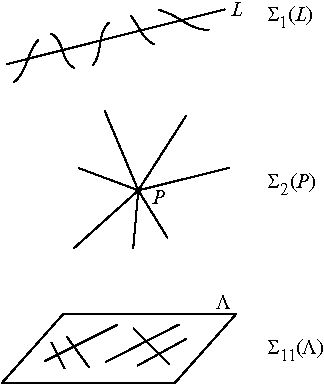
\includegraphics[height=2.7in]{main/Fig12-2}}
\caption{
Schubert cycles in $G(2,4)$:
$\Sigma_{1}(L)$
consists of
lines meeting $L\subset\PP^3$
(top);
$\Sigma_{2}(p)$
consists of
lines passing through $p\in\PP^3$
(middle);
$\Sigma_{1,1}(\Lambda)$
consists of
 lines in the plane $\Lambda\subset
\PP^3$
(bottom).
}
\label{Schubert cycles in G(2,4)}
\end{figure}

Figure~\ref{Schubert cycles in G(2,4)} illustrates some of
the possibilities for lines in $\PP^3` `$.

In particular, if $\sV(p)$ is the vanishing flag for forms of degree $d$
at a point $p\in \PP^{1}$, then
a $\grd$ has ramification sequence (termwise) $\geq \balpha$ at $p$
\index{ramification sequence}%
if and only~if $W$ belongs
to the Schubert variety $\Sigma_{\bbeta}(\sV(p))$, where $\beta_{i} =
\alpha_{\ell-i}$ as above.

For example, the Schubert cycle $\Sigma_{0,\dots,0}$ is the whole
Grassmannian,
\index{Grassmannian}%
and $\Sigma_{1,0,\dots,0}(\cal V)$ is the set of $\ell$-planes that meet
$V_{e-\ell}$ nontrivially, which is
a hyperplane section of the Grassmannian in its 
Pl\"ucker embedding.
\index{Pl\"ucker embedding}%
More generally, the
\emph{special Schubert cycle}
\index{special Schubert cycle}%
\index{Schubert cycle!special}%
$\Sigma_\gamma(\sV) \colonequals  \Sigma_{\gamma,0,\dots, 0}(\sV)$
is the set of $\ell$-planes
meeting  $V_{\gamma-\ell - \beta+1}$ nontrivially.
Since this condition really involves only the single space $U =
V_{e-\ell-\gamma+1}$, we sometimes
 write it
as $\Sigma_\gamma(U)$.

For any Schubert index $\bbeta$, the codimension of $\Sigma_{\bbeta}({\cal
V})$ in $G(\ell, e)$ is $|{\bbeta}|\colonequals  \sum \beta_i$
(Exercise~\ref{codim Schubert}).


\subsection*{Special Schubert cycles and Pieri's formula}

\begin{fact}
The variety of complete flags in $\CC^e$ is rational, and it follows
\index{Schubert cycle!special}%
that the class of $\Sigma_{\bbeta}({\cal V})\subset G$
in the 
Chow ring
\index{Chow ring}%
$A^*(G(\ell, e))$ of the 
Grassmannian
\index{Grassmannian}%
is independent
of the flag $\sV` `$. It is typically denoted $\sigma_{\bbeta}$. Moreover,
the classes $\sigma_{\bbeta}$ form a basis for the Chow ring as a free
abelian group.
\end{fact}

Thus the product $\sigma_\bbeta 
\cdot \sigma_{\smash{\bbeta'}\vphantom\beta}$  % align beta and beta'
is a linear
combination of Schubert classes,
given combinatorially by the \emph{Littlewood--Richardson rule}\emdash see
\index{Littlewood--Richardson rule}%
for example \cite{MR2247964}.
\emph{Pieri's formula} 
\index{Pieri's formula}%
is the special
case of the Littlewood--Richardson rule that expresses the product in
the Chow ring $A^*(G(\ell, e))$ of a special Schubert class with an
arbitrary Schubert class.
In Chapter~\ref{BrillNoetherproofChapter} we will use it to describe
the possible ramification behavior of rational curves with cusps.

\begin{proposition}[Pieri's formula]
\label{Pieri}
If $\sigma_\gamma$ is a 
special Schubert class
\index{Schubert class!special}%
and $\sigma_{\bbeta}$
is an arbitrary Schubert class, then
\index{Schubert class!product of --es}%
$$
\sigma_\gamma \cdot \sigma_{\bbeta} \; = \; \sum \sigma_{\bdelta}
$$
where the sum ranges over all Schubert indices ${\bdelta} = (\delta_1,
\dots \delta_{\ell})$ with
$$
\sum \delta_i = \gamma + \sum \beta_i \quad \text{and} \quad \beta_i
\leq \delta_i \leq \beta_{i-1}\quad \text{ for all } i
.
$$
\end{proposition}

For a proof, see for example \cite[Section 4.2.4]{3264}.

Figure~\ref{intersection product} illustrates the degeneration of
$\Sigma_1\cdot \Sigma_1$ to $\Sigma_2 \cup \Sigma_{1,1}$.

\begin{figure}[b]
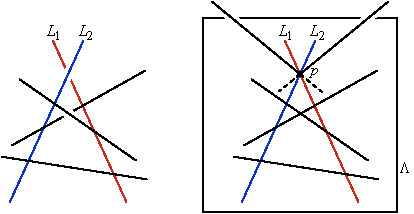
\includegraphics[height=1.8in]{main/Fig12-3}
\caption{When the lines $L_1$ and $L_2$ move to meet each other at $P$
they become coplanar in $\Lambda$,
and the intersection $\Sigma_1(L_1) \cap \Sigma(L_2)$
degenerates to the union $\Sigma_2(P) \cup \Sigma_{1,1}(\Lambda)$.
}
\label{intersection product}
\end{figure}

To understand Proposition~\ref{Pieri}, represent the Schubert class
$\sigma_{\bbeta}$ by 
stacks of coins,
\index{stacks of coins}%
with $\beta_1$ coins in the first
stack, $\beta_2$ coins in the second stack, and so on. We now want to
add a total of $\gamma$ coins to the stacks; we can add any number of
them to any stack (including a stack that was previously empty), with
the one condition that the new height of each stack can't be larger than
the previous height of the stack to its left. This interpretation makes
the following corollary clear:

\begin{corollary}\label{intersection with sigma nonzero}
If $\sigma_\gamma$ is any special Schubert class, $\sigma_{\bbeta}$
is any Schubert class,
and $m\geq 0$ is an integer with $m \gamma + \sum \beta_i \leq \dim
G(\ell, e) = \ell(e-\ell)$, then
$$
(\sigma_\gamma)^l \cdot \sigma_{\bbeta} \neq 0 \in A^*(G(\ell, e), \ZZ).
$$
\end{corollary}

The next result is expressed in terms of the \emph{osculating flag}
\index{osculating flag!defi}%
$\sV = 0\subset
V_1\subset \cdots \subset V_d = \PP^d$
to the rational normal curve $C\subset \PP^{d}$ at a point $p\in C$, which
we will now define. 

\def\tL{\,\widetilde{\!W\!}\,} % avoid superwide tilde
\def\tsV{{\widetilde \sV}}
\def\tV{{\widetilde V}}

Let $\tsV = (\tV_1, \dots, \tV_{d+1})$ be the 
 ramification flag defined previously (leaving
out $\tV_{0}$, which corresponds to the empty projective space), 
and let $V_{i}$ be the projectivization of $\V_{i+1}$. That is,
$V_{i}$ is the projective subspace of dimension $i$ that meets $C$ at $p$
with maximal order of contact.

\begin{proposition}\label{ramification}
Let $C \subset \PP^d$ be a rational normal curve, and $(V_W, \sO_C(1))$
be the $g^r_d$ on $\PP^1$ cut by hyperplanes in $\PP^d$ containing a
plane $W \subset \PP^d$ of dimension $d-r-1$, and write $\sV = 0\subset
V_1\subset \cdots \subset V_d = \PP^d$ for the 
osculating flag
of $C$
at $p$. The ramification sequence $\alpha(V_W, p)$
\index{ramification sequence}%
is determined by the formula
%
$$
W \in \Sigma_{\bfa}({\cal V}) \; \iff \; \alpha_i(V_W, p) \geq
\bfa^*_{r+1-i} = \#\{j\mid a_j\geq r+1-i\}.
$$
\end{proposition}

In other words, the ramification sequence $\alpha(V_W, p)$ of the linear
series $V_W$ at $p$ is exactly the reverse of the transpose of the
Schubert index of the smallest Schubert cycle containing $\tL$, the vector
space associated to $W` `$, in  $G(d-r, d+1)$.

\begin{proof}

The condition $\tL \in \Sigma_{\bfa}({\tsV})$
 means that
$$
\dim \tL \cap \tV_{r+1+i-a_i} \geq i
$$
for each $i$.
It follows that the codimension of the space of hyperplanes containing
$\tL$ has codimension $\leq r-a_i+1$.
since the projective space corresponding to $\tV_{r+i-a_i}$ is the linear
span of the divisor $(r+i-a_i+1)p\subset C$,
a codimension $\leq r-a_i+1$ space of sections of $\tV_{\tL}$  vanishes
to order $\geq r -a_i+1+i$ at $p$.

If we write the distinct orders of vanishing of the sections in
$\tV_{\tL}$ as
$b_0 < b_1<  \cdots < b_r$, we see that $\tL \in \Sigma_{\bfa}$  if
and only~if
$a_i$ of the $b_j$ are $\geq r+i+a_i+1$, that is,
$b_{r-a_i+1}\geq r-a_i+1+i$ or equivalently $\alpha_{r-a_i+1}\geq i$
for each $i$.
Since $\alpha_i\leq \alpha_{i+1} \leq \alpha_r$,
this is equivalent to saying that the number of $\{j \mid \alpha_j \geq
i\}$ is at least $a_i$, or, for the
reverse sequence $\alpha' = \alpha_r \geq \alpha_{r-1} \geq \cdots \geq
0$, that the $a_i$-th term is $\geq i$.
On the other hand $\bfa'_{a_i} = \#\{j\mid a_j \geq a_i\} = i$ since
the sequence $\bfa$ is weakly
decreasing, so $\alpha'$ is termwise $\geq \bfa'$.
\end{proof}

\subsection*{Conclusion}

Using these ideas we  can rephrase and prove Theorem~\ref{transversality
of ramification} in terms of Schubert cycles,
adding the precise condition for the existence of a $\grd$ with prescribed
ramification sequences
at an arbitrary collection of distinct points in $\PP^{1}$:

\begin{theorem}\label{osculating intersection}
Let $p_1,\dots,p_\delta \in C$ be distinct points on a rational normal
curve $C \subset \PP^d` `$, and ${\cal V}^1, \dots, {\cal V}^\delta$ the
corresponding vanishing flags. If ${\bbeta}^1, \dots, {\bbeta}^\delta$
are $\delta$ Schubert indices for $G(d-r, d+1)$, the Schubert cycles
$\Sigma_{{\bbeta}^1}({\cal V}^1), \dots, \Sigma_{{\bbeta}^\delta}({\cal
V}^\delta) \subset G(d-r, d+1)$ intersect properly; that is, the
intersection is either empty or has codimension exactly $\sum_{j
=1}^{\delta}|\bbeta^{j}|$,
the sum of the codimensions of the cycles $\Sigma_{{\bbeta}^j}$. Moreover,
the intersection is nonempty if and only~if
 the intersection product of the classes $[\Sigma_{{\bbeta}^j}]$ is
 nonzero in $A^*(G(d-r, d+1))$.
\end{theorem}


\begin{proof}
If the intersection is empty then the Chow class is 0, so it suffices
to show that the intersection is proper,
and we may assume that it is nonempty. Because the Grassmannian is smooth,
the codimension of the intersection of any subvarieties
 is at most the sum of their codimensions, so it is enough to show that
 the codimension of the
 intersection cannot be too small.

The Schubert cycle $\Sigma_1$ is a hyperplane section of the Grassmannian
$G(d-r, r+1)$, so that if $\Phi \subset G$ is any subvariety of
dimension $m$, its intersection with $m$ Schubert cycles $\Sigma_1$
is nonempty. Thus, if the intersection
$$
X \colonequals  \bigcap_{i=1}^\delta \Sigma_{{\bbeta}^i}({\cal V}^i)
$$
had dimension strictly bigger than the expected
$$
\rho \; \colonequals  \; (r+1)(d-r) - \sum_{i=1}^\delta |{\bbeta}^i|,
$$
we could choose $\rho + 1$ additional points $q_1,\dots,q_{\rho + 1}$
on $C$, with vanishing flags ${\cal V}^1, \dots, {\cal V}^{\rho + 1}$
and the intersection of $X$ with the Schubert cycles $\Sigma_1({\cal
V}^i)$ would still be nonempty.

It thus suffices to show that the intersection is empty if
$$
\sum_{i=1}^\delta |{\bbeta}^i| \; > \; (r+1)(d-r) = \dim G(d-r, d+1).
$$
If on the contrary
$$
W \; \in \; \bigcap_{i=1}^\delta \Sigma_{{\bbeta}^i}({\cal V}^i),
$$
then, by Proposition~\ref{ramification}, the linear series $(W,
\sO_{\PP^{1}}(d))$  would have
ramification of weight $|{\bbeta_i}|$ at $p_i$, and the sum of the
weights would be strictly greater than $(r+1)(d-r)$.
This contradicts the Pl\"ucker formula, Theorem~\ref{Plucker}.
\end{proof}

Using Proposition~\ref{ramification} this result becomes a
characterization of the sets of possible ramification
sequences for linear series at specified points on $\PP^1.$
 Explicitly, suppose we are given a collection of distinct points
 $p_1,\dots,p_\delta \in \PP^1` `$, and for each point $p_i$ a
 ramification sequence
$$
\alpha^i = (\alpha^i_0, \alpha^i_1, \dots, \alpha^i_r) \quad \text{with}
\quad 0 \leq \alpha^i_0 \leq \alpha^i_1 \leq \dots \leq \alpha^i_r
\leq d-r.
$$
Let ${\bbeta}^i$ be this sequence in reverse (and relabelled); that is
$$
{\bbeta}^i \; = \; (\alpha^i_r, \alpha^i_{r-1}, \dots, \alpha^i_1,
\alpha^i_0)
$$
and finally let $\bfb^i$ be the transpose of the Schubert index
${\bbeta}^i` `$.

\begin{corollary}
With $\alpha^i $ and $\bfb^i$ related as above,  there exists a
$g^r_d$ on $\PP^1$ with ramification sequence at $p_i$ equal to
$(\alpha^i_0, \alpha^i_1, \dots, \alpha^i_r)$ if and only~if
$$
\prod_{i=0}^\delta  \sigma_{\bfb^i} \; \neq \; 0 \quad \text{in} \quad
A^*(G(d-r, r+1)).
$$
\end{corollary}

\begin{proof}
If the product is nonzero, Proposition~\ref{ramification} and
Theorem~\ref{osculating intersection} immediately show the existence of
a $g^r_d$ on $\PP^1$ with ramification sequence greater than or equal
to $\alpha^i$ at $p_i$. But by Theorem~\ref{osculating intersection},
the ones with ramification strictly greater than the $\alpha^i$ form
a family of strictly smaller dimension. Thus a general $g^r_d$ with
ramification sequence greater than or equal to $\alpha^i$ at $p_i$
has  ramification sequence exactly equal to $\alpha^i$ at $p_i$.
\end{proof}

We can deduce a result about general secant loci
\index{secant flag}%
strengthening one that
was originally proven in \cite{Griffiths-Harris-BN}:
Given a curve $C \subset \PP^d` `$, we say that a \emph{secant flag}
in $\PP^d$ is a flag
$$
0 \subset V_1 \subset V_2 \subset \dots \subset V_{d-1} \subset V_d
= \PP^d
$$
where each $V_i$ is spanned by its (scheme-theoretic) intersection with
$C$. In other words, there is a sequence of points $p_1, p_2, \dots,
p_{d+1} \in C$ such that
$$
V_i \; = \; \overline{p_1+p_2+ \dots + p_{i+1}}
$$
(An osculating flag is just the special case where all $p_i$ are
equal.) Since any secant flag can specialize to an osculating flag,
we can deduce:

\begin{corollary}\label{secant schubert proper}
Schubert cycles defined relative to \emph{general} secant flags to a
rational normal curve intersect properly.
\end{corollary}

Unlike the case for osculating flags, the hypothesis of generality is
necessary for secant flags; see Exercise~\ref{only general secants}.

\section{Exercises}
\begin{exercise}\label{inseparable Gauss}
Let $k$ be a field of 
characteristic $p$.
\index{positive characteristic}%
Show that every point of the
affine curve $y = x^{p+1}+1$ over $k$ is a flex point.
\end{exercise}

\begin{exercise}\label{2g+2fixedpoints}
Show that if $C$ is a smooth projective curve of genus $g \geq 2$ and
$f : C \to C$ an automorphism fixing $2g+2$ points, then $C$ must be
hyperelliptic
\index{hyperelliptic}%
and $f$ the hyperelliptic involution.

Hint: Since we know that $f$ has finite order, we can take the quotient
$B = C/\langle f \rangle$ of $C$ by the cyclic group $\langle f \rangle$;
apply 
the Riemann--Hurwitz formula
\index{Riemann--Hurwitz formula}%
to the quotient map $C \to B$.
\end{exercise}

\begin{exercise}\label{curve in a product}
Suppose that $C\subset D\times E$ is a curve contained in the product
of smooth curves $D,E$ of genera $g$ and $h$ respectively.
Prove that if the degrees of the projection maps $C \to D$ and $C\to E$
are $d$ and $e$ respectively,
then
$$
p_a(C)\leq (d-1)(e-1) +dg+eh.
$$
Hint:  Use the Hodge index theorem~\ref{hodge index} and the adjunction
\index{Hodge index theorem}%
\index{adjunction formula}%
formula to show that the maximum possible genus of such
a curve $C$ is obtained when $C$ is linearly equivalent to a sum of
fibers of the two projections, in which case the inequality
becomes an equality.
\end{exercise}

\begin{exercise}\label{84(g-1)}
Show that if $C$ is a smooth projective curve of genus $g \geq 2$ then
$$
|\!\Aut C| \leq 84(g-1)
$$

Hint: Since we know that $\Aut C$ has finite order, we can take
the quotient $B = C/\Aut C$ of $C$; again, apply 
the Riemann--Hurwitz formula
\index{Riemann--Hurwitz formula}%
\index{automorphism group!size of}%
to the quotient map $C \to B$. (Warning: the idea is the same as in
Exercise~\ref{2g+2fixedpoints}, but the execution is substantially
more complicated.)
\end{exercise}


\begin{exercise}\label{codim Schubert}
Show that the codimension of $\Sigma_{\bbeta}({\cal V})$ in the
\index{Grassmannian}%
Grassmannian $G$ is equal to $\sum \beta_i$.

Hint: for $\Lambda \in \Sigma_{\bbeta}({\cal V})$, consider bases of
$\Lambda$ such that $\Lambda \cap V_i$ is the span of basis vectors.
\end{exercise}

\begin{exercise}\label{Schubert duality}
Let ${\bbeta}^*$ be
the transpose Schubert index to $\bbeta$.
\begin{enumerate}
\item  Show that $|\bbeta^*| = |\bbeta|$.
\item Show that $(\bbeta^*){\vphantom{\bbeta}}^* = \bbeta$. %align *s
\item Show that the isomorphism $\phi : G(k+1, V) \ruto{\,\cong} 
G(n-k, V^*)$ carries the Schubert cycle $\Sigma_\bbeta({\cal V})$ to the
Schubert cycle $\Sigma_{\bbeta^*}({\cal V}^*)$.
\end{enumerate}
(Of course, the first two parts follow from the third; think of the
first two as warmups.)
\end{exercise}

\begin{exercise}[ramification and osculating planes]\label{osculating
planes}
Let $p\in C\subset \PP^{d}$ be a point on a rational normal curve of
degree $d$, and
let $\Lambda\subset \PP^{d}$ be a $d-r-1$ plane, and let  $\sU
\colonequals (\sO_{\PP^{1}}(d), V)$
be
the  $\grd$,  possibly with basepoints, cut out by hyperplanes containing
$\Lambda$.
Consider the complete flag
$$
U(p) \colonequals  \{U_{1}, \dots, U_{d}\}
$$
of \emph{osculating spaces} at $p$, where $U_{t}$ is the linear span of
\index{osculating space}%
the divisor $tp$ considered
as a subscheme of length $t$ in $C$. Show that the ramification sequence
\index{ramification sequence}%
of $\sU$ at $p$
is determined by the formula
$$
W \in \Sigma_{\bfa}(U(p))
\; \iff \; \alpha_i(\sU, p) \geq \bfa^*_{r+1-i} = \#\{j\mid a_j\geq
r+1-i\}.
$$
In other words, the ramification sequence $\alpha(\sU, p)$ of the linear
series $\sU$ at $p$ is the reverse of the transpose of the Schubert
index of the smallest Schubert cycle containing $L$, the vector
space associated to $\Lambda$, in  $G(d-r, d+1)$. Conclude from
Theorem~\ref{osculating intersection}
that any collection of Schubert cycles associated to osculating flags
of $C$ at distinct points have intersection
that is dimensionally transverse or empty.
\end{exercise}

\begin{exercise}\label{independent secants 0}
Let $C$ be the rational normal curve in $\PP^{r}$. And let $(p_{i},
q_{i})\in  C^{2}$ be $t$ pairs of points, all distinct.
For each $i$, let $S_{i}$ be the Schubert variety of $k$-planes in
$\PP^{r}$ that meet the secant line
$\overline{p_{i}q_{i}}$. Show that if the $p_{i}, q_{i}$ are sufficiently
general, then the intersection
of the $S_{i}$ is dimensionally transverse. Hint: Let each pair of points
come together, and use the result
for the tangent lines, a special case of Theorem~\ref{osculating
intersection}.
\end{exercise}

\begin{exercise}\label{only general secants}
Show by example that Schubert cycles defined relative to arbitrary secant
flags to a rational normal curve may fail to intersect properly. (Hint:
it's enough to look at the case $d=2$ and $r=1$.)
\end{exercise}

\begin{exercise}
We can define the osculating flag to any nondegenerate curve $C \subset
\PP^d$ at any smooth point $p$. If $p$ is an inflection point then
$\overline{mp}$ may not be an $(m-1)$-plane, but we can look at the
nested sequence of subspaces
$$
\{p\} \subset \overline{2p} \subset \overline{3p} \subset \cdots
$$
and pick out exactly the terms whose dimension is strictly greater than
the preceding term; this gives a complete flag
$$
\{p\} \subset \overline{b_2p} \subset \overline{b_3p} \subset \dots
\subset \overline{b_{d+1}p} = \PP^d
.
$$
Show that the sum $\sum b_i - i$ is equal to the weight of the point $p$
as an inflection point of the hyperplane series.
\end{exercise}


\begin{exercise}
The Pl\"ucker formula shows that an elliptic normal curve $E\subset
\PP^{n-1}$ has $n^2$ inflection points. Show that they are
all simple, and that if you choose one as the origin for the group law
on $E$, then
they are the $n$-torsion points of  $E \cong Jac(E)$.

Hint: observe that the inflection points are the points $p \in E$ such
that $\cO_E(np) \cong \cO_E(1)$.
\end{exercise}

\begin{exercise}[Buchweitz]
It was long believed that every semigroup $H \subset \NN$ of finite index
\index{Weierstrass point)}%
$g = \#(\NN \setminus H)$ could occur as the Weierstrass semigroup of
a Weierstrass
point on a curve of genus $g$, but this is not the case. The following
counterexample for a curve of genus 16 was found by Buchweitz
\index{Buchweitz, Ragnar-Olaf}%
(unpublished): Show that on a curve of genus 16 there can be no
Weierstrass point $p$ with ramification sequence
$(0^{12}, 6,7,9,9)$ by showing that there would be too many vanishing
orders at $p$ of quadratic differentials.
 \end{exercise}

%footer for separate chapter files

\ifx\whole\undefined
\makeatletter\def\@biblabel#1{#1]}\makeatother
\gdef\urlhook{\url}
\bibliography{slag}
\bibliographystyle{msribib}


%%%% EXPLANATIONS:

% f and n
% some authors have all works collected at the end

\catcode`\^\active
%if ^ is followed by 
% 1:  print f, gobble the following ^ and the next character
% 0:  print n, gobble the following ^
% any other letter: print letter
\makeatletter
\def^#1{\ifx1#1f\expandafter\@gobbletwo\else
        \ifx0#1n\expandafter\expandafter\expandafter\@gobble\else#1\fi\fi}
\makeatother
\let\moreadhoc\relax
\def\indexintro{%An author's cited works appear at the end of the
%author's entry; for conventions
%see the List of Citations on page~\pageref{loc}.  
%\smallbreak\noindent
The letter `f' after a page number indicates a figure, `n' a footnote.}
\printindex[gen]
%requires makeindex
\end{document}
\else
\fi
